%% Based on a TeXnicCenter-Template by Gyorgy SZEIDL.
%%%%%%%%%%%%%%%%%%%%%%%%%%%%%%%%%%%%%%%%%%%%%%%%%%%%%%%%%%%%%

%----------------------------------------------------------
%
%\documentclass[10pt,a4paper]{exam}
\documentclass[10pt,a4paper,answers]{exam}
%
%----------------------------------------------------------
% This is a sample document for the standard LaTeX Book Class
% Class options
%       --  Body text point size:
%                        10pt (default), 11pt, 12pt
%       --  Paper size:  letterpaper (8.5x11 inch, default)
%                        a4paper, a5paper, b5paper,
%                        legalpaper, executivepaper
%       --  Orientation (portrait is the default):
%                        landscape
%       --  Printside:   oneside, twoside (default)
%       --  Quality:     final(default), draft
%       --  Title page:  titlepage, notitlepage
%       --  Columns:     onecolumn (default), twocolumn
%       --  Start chapter on left:
%                        openright(no, default), openany
%       --  Equation numbering (equation numbers on right is the default):
%                        leqno
%       --  Displayed equations (centered is the default):
%                        fleqn (flush left)
%       --  Open bibliography style (closed bibliography is the default):
%                        openbib
% For instance the command
%          \documentclass[a4paper,12pt,reqno]{book}
% ensures that the paper size is a4, fonts are typeset at the size 12p
% and the equation numbers are on the right side.
%
\usepackage{amsthm}
\usepackage{amsmath}%
\usepackage{amsfonts}%
\usepackage{amssymb}%
\usepackage{graphicx}
\usepackage[pdftex]{epsfig}
\usepackage{cancel}
\newtheorem{proposition}{Proposition}
\newtheorem{definition}{Definition}
%
\usepackage[table,xcdraw]{xcolor}
\usepackage{textcomp,upquote,listings}
\lstset{upquote=true,showstringspaces=false}
%
\usepackage{hyperref}
% Setup TikZ For drawing graphs

\usepackage{tikz}
\usetikzlibrary{arrows}
\tikzset{
    % Define arrow style
    arrow/.style={
           ->,}
}

\usepackage{cancel}
%----------------------------------------------------------
\newcommand{\IfSolution}[1]{#1}

\rhead{\textsf{CS4221/CS5421}}

%%% MVD
\newcommand {\mvd}{\mbox{$\; \rightarrow \! \! \! \! \rightarrow \; $}}

%%%%%%%%%%%%%%%%%%%%%%%%%
%
% THIS IS THE SWITCH FOR SOLUTIONS
% 
%%%%%%%%%%%%%%%%%%%%%%%%%

\newcounter{sol}
\setcounter{sol}{1} % with solutions
%\setcounter{sol}{0} % without solutions
%----------------------------------------------------------
\begin{document}

%%%%%%%%%%%%%%%%%%%%%%
\begin{center}
{\sf\Large\bf Tutorial: Dependencies, entity-relationship modelling and the Chase}
\end{center}

\begin{questions}
\question Consider the entity-relationship diagram of Figure~\ref{fig:er}. 

\begin{figure}[h]
\label{fig:er}
\begin{center}
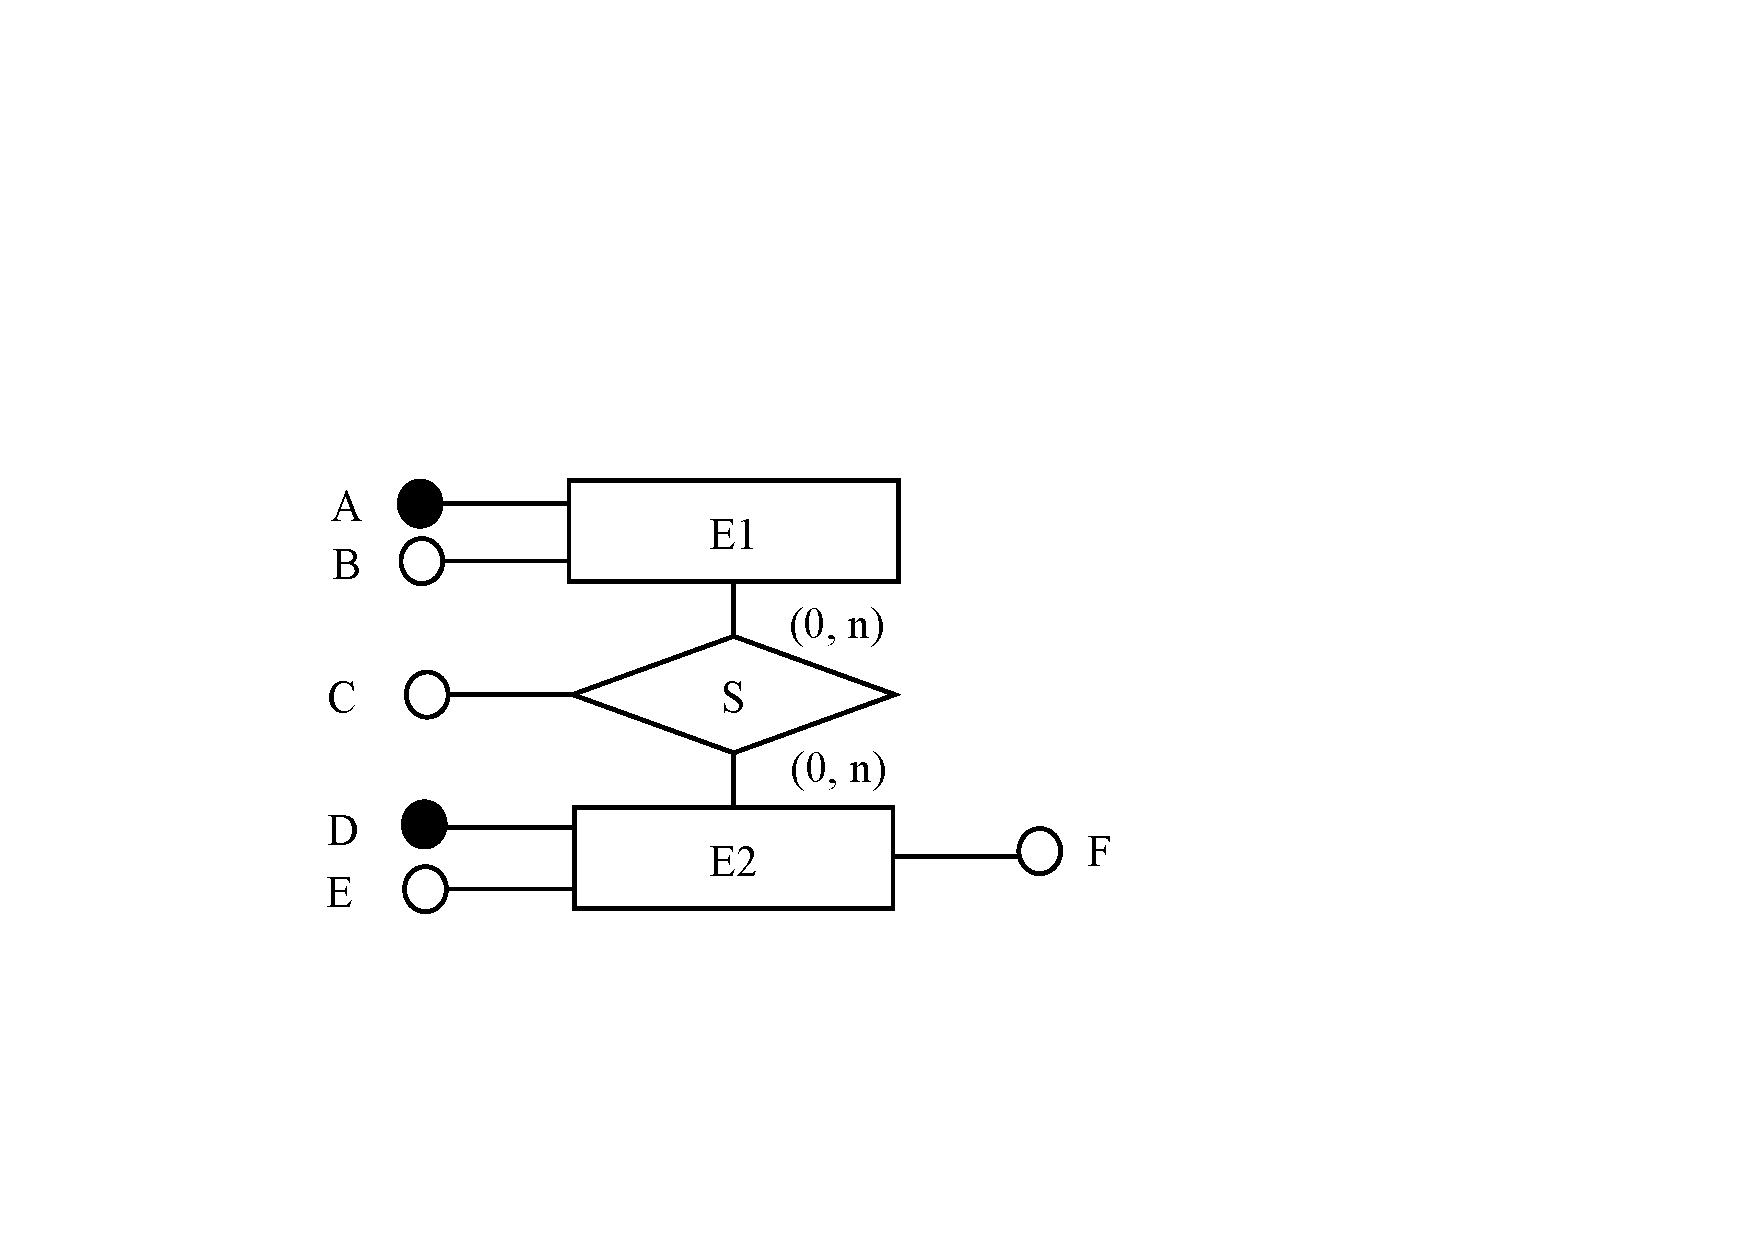
\includegraphics[width=0.5\linewidth]{images/er}
\end{center}
\caption{Entity-relationship diagram.}
\end{figure}

\begin{parts}
\part Without other knowledge than that captured by the entity-relationship diagram, what are the functional and multivalued dependencies?


\begin{solution}
The entity-relationship diagram tells us the following functional dependencies.

\[\Sigma=\{\{A\}\rightarrow\{B\}, \{D\}\rightarrow\{E, F\}, \{A, D\}\rightarrow\{C\}\}\]

Multivalued dependencies depend on the translation of this design into tables. The entity-relationship diagram and its translation will only result in ``not interesting'' multi-valued dependencies, that is dependencies that are trivial or correspond to the table or the functional dependencies. If we canonically translate this design into three tables, we have $\{A\} \mvd \{B\}$ and $\{D\} \mvd \{E,F\}$ and many more (none of them being useful for normalisation), for instance.

Note that additional knowledge of the application could tell us additional functional and multivalued dependencies not captured by the design. 

For instance, we could know that $\{E\}\rightarrow\{F\}$ (which would suggest that the entity-relationship design is probably missing entities and relationships that have been merged too early), which we could use to produce a design in the Boyce-Codd normal by splitting the table $R_3(D, E, F)$ into two tables $R_{3.2}(\underline{D}, E)$ and $R_{3.2}(\underline{E}, F)$.


For instance, we could know that $\{E\}\mvd\{F\}$, which we could use to produce a design in the fifth normal by splitting the table $R_3(D, E, F)$ into two tables $R_{3.2}(\underline{D}, E)$ and $R_{3.2}(\underline{E, F})$.


\end{solution}
\end{parts}


\question Consider the relational schema $R=\{A, B, C, D, E\}$ with the following set of functional and multi-valued dependencies.

$\Sigma=\{ \{C\}\rightarrow\{A\},  \{D\} \rightarrow \{D, B\}, \{B\} \rightarrow \{E\}, \{E\} \mvd \{A, D\}, \{A, B, D\} \rightarrow \{A, B, C, D\}, \{B\} \rightarrow \{D\}\}$

\begin{parts}
\part Prove that $\{E\} \rightarrow \{D\}$ using the Armstrong and multi-valued dependencies axioms.

\begin{solution}
\begin{enumerate}
\item We know that $\{E\} \mvd \{A, D\}$.
\item We know that $\{B\} \rightarrow \{D\}$.
\item We see that  $\{D\} \subset \{A, D\}$.
\item We see that  $\{B\} \cap \{A, D\} = \emptyset$.
\item Therefore $\{E\} \rightarrow \{D\}$ by Coalescence of (1), (2), (3) and (4).
\item[] Q.E.D.
\end{enumerate}

Try the same question with the Chase (answer not provided).
\end{solution}

\end{parts}

\question Consider the  relation $R(A, B, C, D, E, G)$ with the following set, $F$, of functional and multi-valued dependencies. 

$F=\{ \{A, B\} \rightarrow \{C\}, \{A, B\} \mvd \{E\}, \{C, D\} \mvd \{A, B\}\}$

\begin{parts}
	\part Prove that the decomposition of $R$ into $R_1(A, B, C, D, G)$ and $R_2(C, D, E)$ is lossless using the Chase algorithm (as shown in the lecture).
\end{parts}

\begin{solution}
	\begin{enumerate}
		\item Initial table.
		\begin{center}
			\centering
			\begin{tabular}{|c|c|c|c|c|c|}
				\hline
				\rowcolor[HTML]{EFEFEF} 
				\textbf{A} & \textbf{B} & \textbf{C} & \textbf{D} & \textbf{E} & {\color[HTML]{333333} \textbf{G}} \\ \hline
				a1         & b1         & c1         & d1         & e1         & g1                                \\ \hline
				a2         & b2         & c2         & d2         & e2         & g2                                \\ \hline
			\end{tabular}
		\end{center}
		\item We want to chase $\{C, D\} \mvd \{E\}$, make $C$ and $D$ values the same.
		\begin{center}
			\centering
			\begin{tabular}{|c|c|c|c|c|c|}
				\hline
				\rowcolor[HTML]{EFEFEF} 
				\textbf{A} & \textbf{B} & \textbf{C} & \textbf{D} & \textbf{E} & {\color[HTML]{333333} \textbf{G}} \\ \hline
				a1         & b1         & \textbf{c1}         & \textbf{d1}         & e1         & g1                                \\ \hline
				a2         & b2         & \textbf{c1}         & \textbf{d1}         & e2         & g2                                \\ \hline
			\end{tabular}
		\end{center}
		\item Apply $\{C, D\} \mvd \{A, B\}$ by copying two t-uples that have the same $C$ and $D$ values but swapping their $A$ and $B$ values.
		\begin{center}
			\centering
			\begin{tabular}{|c|c|c|c|c|c|}
				\hline
				\rowcolor[HTML]{EFEFEF} 
				\textbf{A}               & \textbf{B}              & \textbf{C}              & \textbf{D}              & \textbf{E}              & {\color[HTML]{333333} \textbf{G}} \\ \hline
				a1                       & b1                      & c1                      & d1                      & e1                      & g1                                \\ \hline
				a2                       & b2                      & c1                      & d1                      & e2                      & g2                                \\ \hline
				\multicolumn{1}{|l|}{\textbf{a2}} & \multicolumn{1}{l|}{\textbf{b2}} & \multicolumn{1}{l|}{c1} & \multicolumn{1}{l|}{d1} & \multicolumn{1}{l|}{e1} & \multicolumn{1}{l|}{g1}           \\ \hline
				\multicolumn{1}{|l|}{\textbf{a1}} & \multicolumn{1}{l|}{\textbf{b1}} & \multicolumn{1}{l|}{c1} & \multicolumn{1}{l|}{d1} & \multicolumn{1}{l|}{e2} & \multicolumn{1}{l|}{g2}           \\ \hline
			\end{tabular}
		\end{center}
		
		\item Apply $\{A, B\} \mvd \{E\}$ by copying two t-uples by copying two t-uples that have the same $A$ and $B$ values but swapping their $A$ and $E$ values.
		\begin{center}
			\centering
			\begin{tabular}{|l|l|l|l|l|l|}
				\hline
				\rowcolor[HTML]{EFEFEF} 
				\multicolumn{1}{|c|}{\cellcolor[HTML]{EFEFEF}\textbf{A}} & \multicolumn{1}{c|}{\cellcolor[HTML]{EFEFEF}\textbf{B}} & \multicolumn{1}{c|}{\cellcolor[HTML]{EFEFEF}\textbf{C}} & \multicolumn{1}{c|}{\cellcolor[HTML]{EFEFEF}\textbf{D}} & \multicolumn{1}{c|}{\cellcolor[HTML]{EFEFEF}\textbf{E}} & \multicolumn{1}{c|}{\cellcolor[HTML]{EFEFEF}{\color[HTML]{333333} \textbf{G}}} \\ \hline
				\multicolumn{1}{|c|}{a1}                                 & \multicolumn{1}{c|}{b1}                                 & \multicolumn{1}{c|}{c1}                                 & \multicolumn{1}{c|}{d1}                                 & \multicolumn{1}{c|}{e1}                                 & \multicolumn{1}{c|}{g1}                                                        \\ \hline
				\multicolumn{1}{|c|}{a2}                                 & \multicolumn{1}{c|}{b2}                                 & \multicolumn{1}{c|}{c1}                                 & \multicolumn{1}{c|}{d1}                                 & \multicolumn{1}{c|}{e2}                                 & \multicolumn{1}{c|}{g2}                                                        \\ \hline
				a2                                                       & b2                                                      & c1                                                      & d1                                                      & e1                                                      & g1                                                                             \\ \hline
				a1                                                       & b1                                                      & c1                                                      & d1                                                      & e2                                                      & g2                                                                             \\ \hline
				a1                                                       & b1                                                      & c1                                                      & d1                                                      & \textbf{e2}                                                      & g1                                                                             \\ \hline
				a2                                                       & b2                                                      & c1                                                      & d1                                                      & \textbf{e1}                                                      & g2                                                                             \\ \hline
				a2                                                       & b2                                                      & c1                                                      & d1                                                      & \textbf{e2}                                                      & g1                                                                             \\ \hline
				a1                                                       & b1                                                      & c1                                                      & d1                                                      & \textbf{e1}                                                      & g2                                                                             \\ \hline
			\end{tabular}
		\end{center}
		
		\item Applying $\{A,B\} \rightarrow {C}$ do not change the table.
		\item Sort the table and proved that $\{C, D\} \mvd \{E\}$
		\begin{center}
			\centering
			\begin{tabular}{|l|l|l|l|l|l|}
				\hline
				\rowcolor[HTML]{EFEFEF} 
				\multicolumn{1}{|c|}{\cellcolor[HTML]{EFEFEF}\textbf{A}} & \multicolumn{1}{c|}{\cellcolor[HTML]{EFEFEF}\textbf{B}} & \multicolumn{1}{c|}{\cellcolor[HTML]{EFEFEF}\textbf{C}} & \multicolumn{1}{c|}{\cellcolor[HTML]{EFEFEF}\textbf{D}} & \multicolumn{1}{c|}{\cellcolor[HTML]{EFEFEF}\textbf{E}} & \multicolumn{1}{c|}{\cellcolor[HTML]{EFEFEF}{\color[HTML]{333333} \textbf{G}}} \\ \hline
				\multicolumn{1}{|c|}{a1}                                 & \multicolumn{1}{c|}{b1}                                 & \multicolumn{1}{c|}{c1}                                 & \multicolumn{1}{c|}{d1}                                 & \multicolumn{1}{c|}{e1}                                 & \multicolumn{1}{c|}{g1}                                                        \\ \hline
				\multicolumn{1}{|c|}{a1}                                 & \multicolumn{1}{c|}{b1}                                 & \multicolumn{1}{c|}{c1}                                 & \multicolumn{1}{c|}{d1}                                 & \multicolumn{1}{c|}{e2}                                 & \multicolumn{1}{c|}{g1}                                                        \\ \hline
				a2                                                       & b2                                                      & c1                                                      & d1                                                      & e1                                                      & g2                                                                             \\ \hline
				a2                                                       & b2                                                      & c1                                                      & d1                                                      & e2                                                      & g2                                                                             \\ \hline
				a2                                                       & b2                                                      & c1                                                      & d1                                                      & e1                                                      & g1                                                                             \\ \hline
				a2                                                       & b2                                                      & c1                                                      & d1                                                      & e2                                                      & g1                                                                             \\ \hline
				a1                                                       & b1                                                      & c1                                                      & d1                                                      & e2                                                      & g2                                                                             \\ \hline
				a1                                                       & b1                                                      & c1                                                      & d1                                                      & e1                                                      & g2                                                                             \\ \hline
			\end{tabular}
		\end{center}
	\end{enumerate}
	
\end{solution}

\question Consider the  relation $R(A, B, C, D, E, F, G)$ with the following set, $\Sigma$, of functional dependencies. 

$\Sigma = \{ \{A, B\} \rightarrow \{C\}, \{C\} \rightarrow \{D, E\}, \{E\} \rightarrow \{D\}, \{F\} \rightarrow \{G\}\}$

\begin{parts}
	\part Prove that the decomposition of $R$ into $R_1(A, B, C, D, E)$ and $R_2(A, B, F, G)$ is lossless using the Chase algorithm (as shown in the lecture).
	\begin{solution}
			\begin{enumerate}
			\item Initial table.
			\begin{center}
				\centering
				\begin{tabular}{|c|c|c|c|c|c|c|}
					\hline
					\rowcolor[HTML]{EFEFEF} 
					\textbf{A} & \textbf{B} & \textbf{C} & \textbf{D} & \textbf{E} & {\color[HTML]{333333} \textbf{F}} & \textbf{G} \\ \hline
					a1         & b1         & c1         & d1         & e1         & f1         & g1                       \\ \hline
					a2         & b2         & c2         & d2         & e2         & f2         & g2                       \\ \hline
				\end{tabular}
			\end{center}
			\item We want to chase $\{A, B\} \mvd \{C,D,E\}$, make $A$ and $B$ values the same.
			
			\begin{center}
				\centering
				\begin{tabular}{|c|c|c|c|c|c|c|}
					\hline
					\rowcolor[HTML]{EFEFEF} 
					\textbf{A} & \textbf{B} & \textbf{C} & \textbf{D} & \textbf{E} & {\color[HTML]{333333} \textbf{F}} & \textbf{G} \\ \hline
					\textbf{a1}         & \textbf{b1}         & c1         & d1         & e1         & f1         & g1                       \\ \hline
					\textbf{a1}         & \textbf{b1}         & c2         & d2         & e2         & f2         & g2                       \\ \hline
				\end{tabular}
			\end{center}
		
		\item Apply $\{A, B\} \rightarrow \{C\}$, make $C$ with the same $A$ and $B$ values the same.
		
		\begin{center}
			\centering
			\begin{tabular}{|c|c|c|c|c|c|c|}
				\hline
				\rowcolor[HTML]{EFEFEF} 
				\textbf{A} & \textbf{B} & \textbf{C} & \textbf{D} & \textbf{E} & {\color[HTML]{333333} \textbf{F}} & \textbf{G} \\ \hline
				a1         & b1         & \textbf{c1}         & d1         & e1         & f1         & g1                       \\ \hline
				a1         & b1         & \textbf{c1}         & d2         & e2         & f2         & g2                       \\ \hline
			\end{tabular}
		\end{center}
		\item Apply $\{C\} \rightarrow \{D,E\}$, make $D$ and $E$ with the same $C$ values the same.
	
	\begin{center}
		\centering
		\begin{tabular}{|c|c|c|c|c|c|c|}
			\hline
			\rowcolor[HTML]{EFEFEF} 
			\textbf{A} & \textbf{B} & \textbf{C} & \textbf{D} & \textbf{E} & {\color[HTML]{333333} \textbf{F}} & \textbf{G} \\ \hline
			a1         & b1         & c1         & \textbf{d1}         & \textbf{e1}         & f1         & g1                       \\ \hline
			a1         & b1         & c1         & \textbf{d1}         & \textbf{e1}         & f2         & g2                       \\ \hline
		\end{tabular}
	\end{center}

	\item Applying $\{E\} \rightarrow \{D\}$ does not change the table.
	
	\item Applying $\{F\} \rightarrow \{G\}$ does not change the table.
	\item Proved that $\{A, B\} \mvd \{C,D,E\}$.
		\end{enumerate}
	\end{solution}
\end{parts}


\question Consider the  relation $R(A, B, C, D, E)$ with the following set, $\Sigma$, of functional dependencies. 

$\Sigma = \{ \{A\} \rightarrow \{B, C\}, \{B\} \rightarrow \{A\}, \{C\} \rightarrow \{D\}\}$

\begin{parts}
	\part Check whether the decomposition of $R$ into $R_1(A, E)$, $R_2(C, D)$ and $R_3 (A, B, C)$ is lossless or lossy using the Chase algorithm with the distinguished attributes.
	\begin{solution}
			\begin{enumerate}
				\item Initial table.
				\begin{center}
					\centering
				\begin{tabular}{|c|c|c|c|c|c|}
					\hline
					\rowcolor[HTML]{EFEFEF} 
					& \textbf{A} & \textbf{B} & \textbf{C} & \textbf{D} & \textbf{E} \\ \hline
					$R_1$ & a          &            &            &            & a          \\ \hline
					$R_2$ &            &            & a          & a          &            \\ \hline
					$R_3$ & a          & a          & a          &            &            \\ \hline
				\end{tabular}
				\end{center}
				\item Apply $\{A\} \rightarrow \{B, C\}$
			\begin{center}
				\centering
				\begin{tabular}{|c|c|c|c|c|c|}
					\hline
					\rowcolor[HTML]{EFEFEF} 
					& \textbf{A} & \textbf{B} & \textbf{C} & \textbf{D} & \textbf{E} \\ \hline
					$R_1$ & a          &     \textbf{a}      &      \textbf{a}      &            & a          \\ \hline
					$R_2$ &            &            & a          & a          &            \\ \hline
					$R_3$ & a          & a          & a          &            &            \\ \hline
				\end{tabular}
			\end{center}
			\item Applying $\{B\} \rightarrow \{A\}$ does not change the table.
			\item Apply $\{C\} \rightarrow \{D\}$
			\begin{center}
				\centering
				\begin{tabular}{|c|c|c|c|c|c|}
					\hline
					\rowcolor[HTML]{EFEFEF} 
					& \textbf{A} & \textbf{B} & \textbf{C} & \textbf{D} & \textbf{E} \\ \hline
					$R_1$ & a          &     a      &      a      &     \textbf{a}       & a          \\ \hline
					$R_2$ &            &            & a          & a          &            \\ \hline
					$R_3$ & a          & a          & a          &       \textbf{a}       &            \\ \hline
				\end{tabular}
			\end{center}
		
			\item $R_1$ has distinguished variables in all of the columns, therefore the decomposition is lossless.
			\end{enumerate}
	\end{solution}
\end{parts}


\end{questions}

\end{document}